% !TeX spellcheck = es_ES
\documentclass[12pt, titlepage]{article}
\usepackage[utf8]{inputenc}
\usepackage[spanish]{babel}
\usepackage{float}
\usepackage[letterpaper, margin=2.5cm]{geometry}
\usepackage[nottoc,notlot,notlof]{tocbibind} % Hace que se agregen las referencias al indice
\usepackage{url}
\usepackage{graphicx} 
\usepackage{listings}
\usepackage{color}
\definecolor{dkgreen}{rgb}{0,0.6,0}
\definecolor{gray}{rgb}{0.5,0.5,0.5}
\definecolor{mauve}{RGB}{253,151,31}

\lstset{frame=tb,
    language=Sql,
    aboveskip=3mm,
    belowskip=3mm,
    showstringspaces=false,
    columns=flexible,
    basicstyle={\small\ttfamily},
    numbers=none,
    numberstyle=\tiny\color{gray},
    keywordstyle=\color{blue},
    commentstyle=\color{dkgreen},
    stringstyle=\color{mauve},
    breaklines=true,
    breakatwhitespace=true,
    tabsize=2,
    morekeywords={use}
}

\title{Reporte: Práctica 6}
\author{Carlos Tonatihu Barrera Pérez \\ Profesor: Hernández Contreras Euler \\ Bases de Datos \\ Grupo: 2CM1 }

\begin{document}
	\maketitle
	\tableofcontents
	\section{Marco Teórico}
	Las vistas son relaciones que no forman parte del modelo lógico pero que se hacen visibles a los usuarios como relaciones virtuales. Además, es posible definir muchas vistas de cualquier conjunto de relaciones.\cite{LIBRO}
	
	Las vistas se definen mediante la siguiente estructura:
	\begin{center}
		\textbf{create view} \textit{nombre\_vista} as $<$expresión de consulta$>$
	\end{center}
	Los elementos que conforman esta estructura son:
	\begin{itemize}
		\item \textbf{create view} es la instrucción que se usa para la creación de vistas.
		\item \textit{nombre\_vista} representa el nombre que puede adoptar esta vista.
		\item $<$expresión de consulta$>$ hace alusión a cualquier expresión legal de consulta.
	\end{itemize}
	Una vez creada la vista se puede utilizar para hacer referencia a la relación virtual que genera
	
	El siguiente diagrama representa la base de datos con la que se trabajo en esta práctica. Las vistas pueden aparecer en cualquier lugar en el que puedan hacerlo los nombre de las relaciones, siempre y cuando no se ejecuten sobre las vistas operaciones de actualización.
	 \begin{figure}[H]
		\begin{center}
			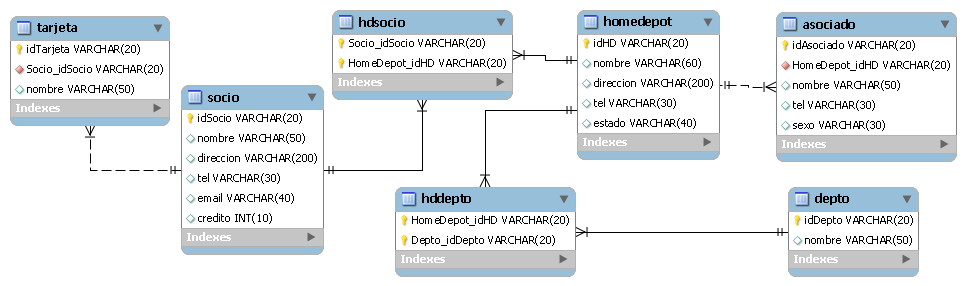
\includegraphics[width=16cm, height=5cm]{img/home.png}
			\label{fig:home}
		\end{center}
	\end{figure}
	Las vistas nos permiten ocultar ciertos datos a los usuarios por lo que representan un nivel de seguridad básico.
	\section{Desarrollo}
	Al igual que en las practicas anteriores en esta se trabajo con una base de datos ya existente en la que se trabajaron los siguientes ejercicios de vistas.
	
	Primero se creo una vista para mostrar el nombre del socio y la tarjeta asignada.
	\begin{figure}[H]
		\begin{center}
			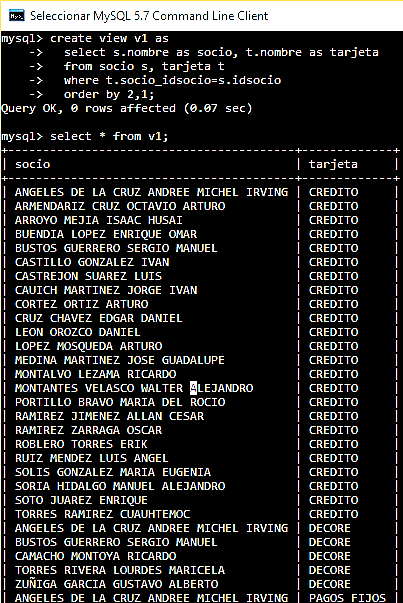
\includegraphics[width=12cm, height=14cm]{img/v1.png}
			\label{fig:v1}
			\caption{Esta vista regreso 48 resultados}
		\end{center}
	\end{figure}
\newpage
	La segunda vista implico mostrar el nombre de asociado y su respectivo teléfono.
	\begin{figure}[H]
		\begin{center}
			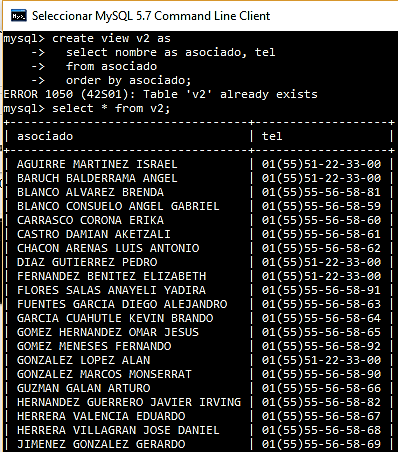
\includegraphics[width=10cm, height=9cm]{img/v2.png}
			\label{fig:v2}
			\caption{Esta vista regreso 49 resultados}
		\end{center}
	\end{figure}
	
	A continuación se creo una vista para el nombre del socio y su email.
	\begin{figure}[H]
		\begin{center}
			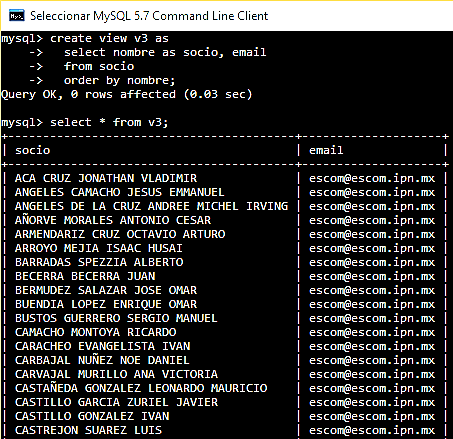
\includegraphics[width=10cm, height=8.5cm]{img/v3.png}
			\label{fig:v3}
			\caption{Esta vista regreso 189 resultados}
		\end{center}
	\end{figure}
	
	La siguiente vista permitió imprimir el nombre de la sucursal y el estado donde se ubica.
	\begin{figure}[H]
		\begin{center}
			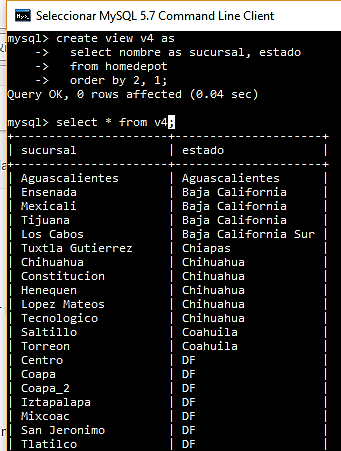
\includegraphics[width=8cm, height=8.5cm]{img/v4.png}
			\label{fig:v4}
			\caption{Esta vista regreso 63 resultados}
		\end{center}
	\end{figure}
	
	Después, se diseño la vista que permite mostrar el nombre de socio y su monto de crédito.
	\begin{figure}[H]
		\begin{center}
			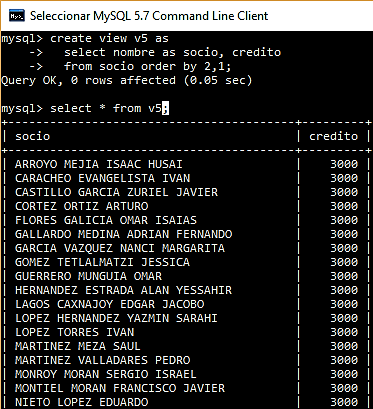
\includegraphics[width=8cm, height=9cm]{img/v5.png}
			\label{fig:v5}
			\caption{Esta vista regreso 189 resultados}
		\end{center}
	\end{figure}
	La siguiente vista muestra el nombre del asociado y su genero.
		\begin{figure}[H]
		\begin{center}
			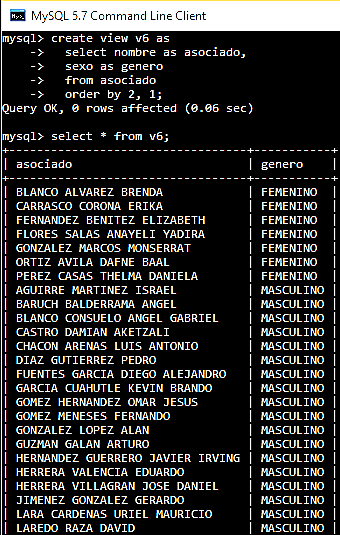
\includegraphics[width=8.5cm, height=9cm]{img/v6.png}
			\label{fig:v6}
			\caption{Esta vista regreso 49 resultados}
		\end{center}
	\end{figure}
	Luego se creo la vista para imprimir el nombre de la sucursal y su departamento.
	\begin{figure}[H]
		\begin{center}
			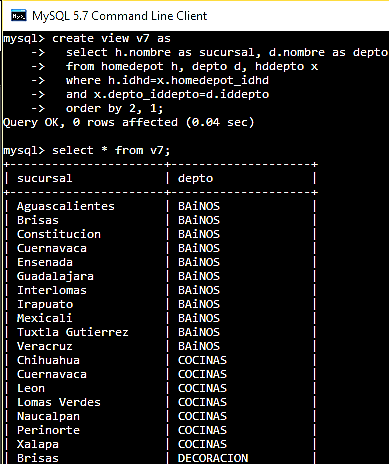
\includegraphics[width=8cm, height=8.5cm]{img/v7.png}
			\label{fig:v7}
			\caption{Esta vista regreso 132 resultados}
		\end{center}
	\end{figure}
	
	A continuación se hizo la vista para desplegar el nombre del socio y su dirección.
	\begin{figure}[H]
		\begin{center}
			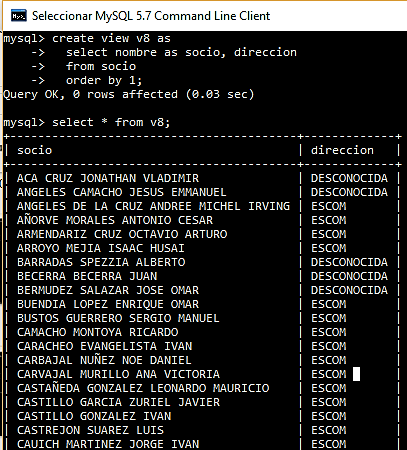
\includegraphics[width=8cm, height=8.5cm]{img/v8.png}
			\label{fig:v8}
			\caption{Esta vista regreso 189 resultados}
		\end{center}
	\end{figure}
	La siguiente vista fue similar pero mostrando el nombre de la sucursal y su directorio.
	\begin{figure}[H]
		\begin{center}
			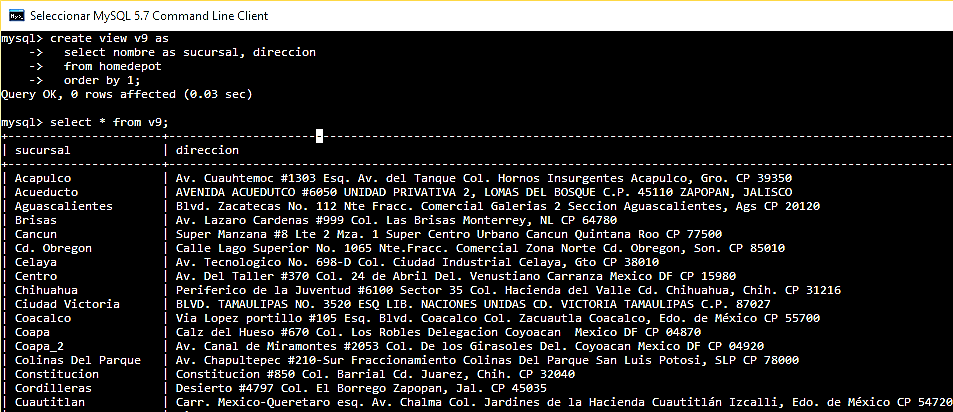
\includegraphics[width=16cm, height=9cm]{img/v9.png}
			\label{fig:v9}
			\caption{Esta vista regreso 63 resultados}
		\end{center}
	\end{figure}
	El nombre del socio y su teléfono se muestran gracias a la siguiente vista.
	\begin{figure}[H]
		\begin{center}
			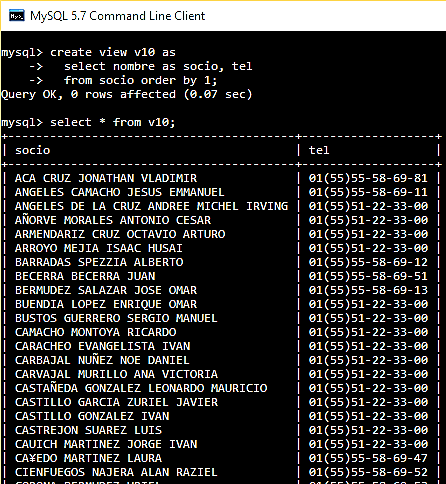
\includegraphics[width=9cm, height=8.5cm]{img/v10.png}
			\label{fig:10}
			\caption{Esta vista regreso 63 resultados}
		\end{center}
	\end{figure}
	Después, se hizo la vista para mostrar el nombre de un asociado y su sucursal.
	\begin{figure}[H]
		\begin{center}
			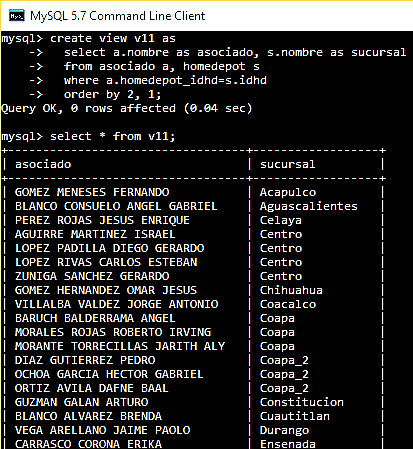
\includegraphics[width=10cm, height=9cm]{img/v11.png}
			\label{fig:11}
			\caption{Esta vista regreso 49 resultados}
		\end{center}
	\end{figure}
	
	Para finalizar este conjunto de ejercicios se creo la vista para mostrar el nombre del socio.
	\begin{figure}[H]
		\begin{center}
			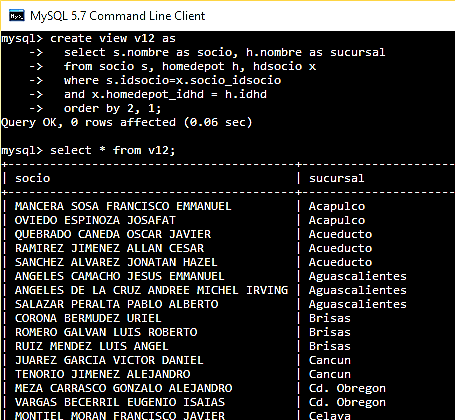
\includegraphics[width=10cm, height=10cm]{img/v12.png}
			\label{fig:12}
			\caption{Esta vista regreso 199 resultados}
		\end{center}
	\end{figure}
	
	Las siguientes consultas se hicieron apoyándose en las vistas antes creadas para simplificar su descripción.
	
	Lo primero fue mostrar el nombre del asociado, el genero y la sucursal pero solo de los que se apellidan García. Para realizar esto se usaron la vista 6  y 11.
	\begin{figure}[H]
		\begin{center}
			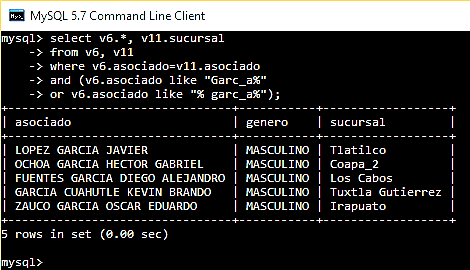
\includegraphics[width=10cm, height=5.5cm]{img/v13.png}
			\label{fig:13}
			\caption{Esta vista regreso 5 resultados}
		\end{center}
	\end{figure}
	La vista cuatro y nueve fueron usadas para desplegar el nombre de la sucursal, el estado y su dirección.
	\begin{figure}[H]
		\begin{center}
			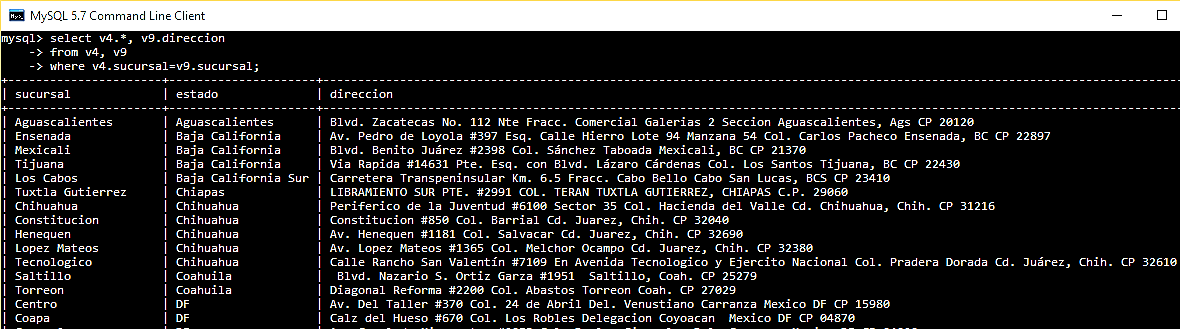
\includegraphics[width=16cm, height=8cm]{img/v14.png}
			\label{fig:14}
			\caption{Esta vista regreso 63 resultados}
		\end{center}
	\end{figure}
	A continuación se mostraron el nombre de los socios que se apellidan Pérez con ayuda de las vistas 5 y 10.
		\begin{figure}[H]
		\begin{center}
			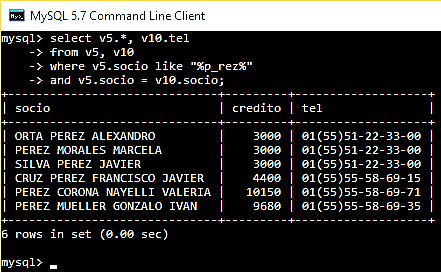
\includegraphics[width=11cm, height=8.5cm]{img/v15.png}
			\label{fig:15}
			\caption{Esta vista regreso 6 resultados}
		\end{center}
	\end{figure}
	 
	Después, se mostró el nombre de los socios, su dirección y sucursal donde están inscritos utilizando las vistas ocho y doce.
		\begin{figure}[H]
		\begin{center}
			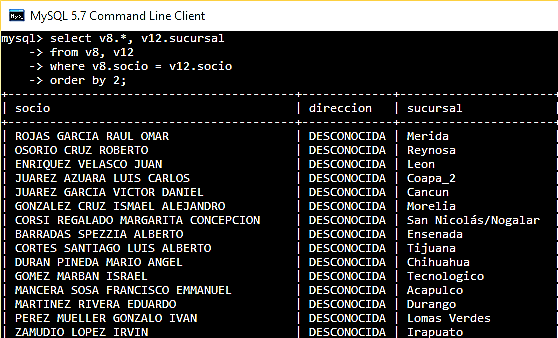
\includegraphics[width=14cm, height=8cm]{img/v16.png}
			\label{fig:16}
			\caption{Esta vista regreso 199 resultados}
		\end{center}
	\end{figure}
	
	Finalmente se usaron las vistas cuatro y once para imprimir el nombre de las sucursales, estado y el nombre de sus asociados pero solo de aquellas ubicadas en el Estado de México.
	\begin{figure}[H]
		\begin{center}
			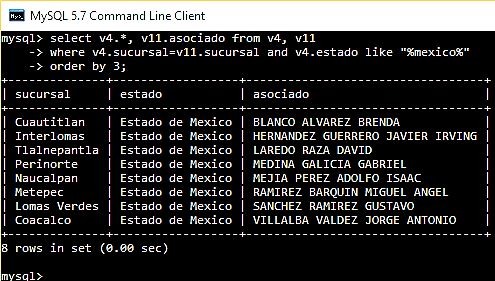
\includegraphics[width=12cm, height=7cm]{img/v17.png}
			\label{fig:17}
			\caption{Esta vista regreso 8 resultados}
		\end{center}
	\end{figure}
	
	
	\section{Conclusiones}
	Como se puede observar en la práctica las vistas son una nueva herramienta que podremos usar para facilitar las consultas a la base de datos ya que como se mostró en prácticas anteriores estas pueden llegar a ser extremadamente largas e incluso podrían volverse confusas por lo que con las vistas podremos obtener un nuevo nivel de abstracción el cual nos podrá facilitar el trabajo aunque hay que mencionar que se debe de tener mucho cuidado para no equivocarse desde la creación de las vistas ya que a la larga esto afectara las subsecuentes consultas que utilicen dicha vista.
	\bibliography{bibliografia} 
	\bibliographystyle{ieeetr}
\end{document}